\chapter{Introduction to Optimization}

\section{What is Optimization?}

In the 1940s as British military leaders asked scientists and engineers to
analyze problems such as where to deploy radar for the cheapest and with the
most coverage. This resulted in the field of Operations Research (OR). 
Optimization is simply an alternate name for Operations Research. It is also
known as mathematical optimization, management science, and decision science.
To be more specific, optimization is a discipline of applying advanced analytical
methods to help make better decisions. It also has ties to other fields such as 
computer science, economics, and many more.

\subsection*{Common Usage}

Common use cases of optimization nowadays is in scheduling and production planning.
For example, suppose that, in order to create a product, you have to produce 
multiple parts in order to build said product. An optimization problem for this
scenario could be how to arrange the sequence of the parts production such that
the amount of change-over time is minimized.

Later on, we will have a closer look at production planning to better
understand the various terms and concepts in optimization.

\section{Mathematical Programming}

One of the first concepts to understand in optimization is mathematical
programming. While it has the word programming it in, it is not the same as 
computer programming. Instead, programming in this case has a closer meaning
to \textit{planning} that concerns optimizing for something.

In order to mathematically \textit{program} a real-world object, it must first be
represented in math$-$a mathematical model. A model is a
structure that is built to replicate the features and characteristics of a
real-world object. This is done in order to learn more about said object and
reveal relationships that may not be so apparent. This gives us a greater
understanding of the object and allows the problem to be analyzed mathematically.
Additionally, experimentation with the model is also possible even if
experimentation on the real-world object might be impossible. You probably
wouldn't want to have to travel to a blackhole to conduct experiments.

In this course, only \textbf{linear} and \textbf{deterministic} models are
considered. This means that linearity assumptions will be used which makes the
models much easier to solve. \textbf{Non-linear} models do exist but are much
more difficult to solve than linear ones. Additionally, parameters here are
\textit{constant}. \textbf{Non-deterministic} or stochastic models where the 
parameters are random also do exist but we can solve it using probability and
expectation.

\section{Problem-Solving with Optimization}

Optimization can be simplified down to three simple steps: \textit{formulation, 
solving, and evaluation}. Currently, there are many methods used to solve
optimization problems. In this course, we will mainly focus on the simplex method.
Once the solution has been computed, it is evaluated on how reasonable it is and
if it is missing any important requirement. As for formulation, we will get it
a bit more detail

\subsection*{Formulation}

Essentially, any physical problem must be translated into a mathematical and
quantitative model in order for it to be solved. This model can be an a simplication
of the real situation and some unimportant elements could be ignored.

To formulate a problem, one must identify its \textbf{decision variables}. These
are the variables that will be changed in order to achieve the goal. Next, one 
must come up with an \textbf{objective function}. This represents the \textit{quality}
of our solution. To ensure that the objective function is feasible, it is
subjected to \textbf{constraints}. These are the mathematical representations of 
real-world limitations present in the model. A constraint that is common in many 
real-world optimization problems is the \textbf{sign-resriction constraint} where 
it usually restricts the decision variable to be non-negative since there is no 
negative count in the real world. The constraint is in the form of either an equation
or an inequality.

\begin{example}
A chocolate company sells to kinds of chocolate: A and B. The 
ingredients used in both types are milk and cocoa powder. Each type 
has its own ratio of milk to cocoa powder where chocolate A's ratio 
is 1:4 while B's is 1:1. Additionally, A and B makes \$2 and \$1 
net profit respectively. The company has 40 units of milk and 100 units 
of cocoa powder. In order to maximize profit, how many units of each 
type of chocolate must the company produce?

\textbf{Formulation. } Let $x$ and $y$ be the units of chocolate A and chocolate B
produced respectively. Let us define the objective function $f$ to represent the 
net profit from selling the chocolate.

\begin{equation}\label{chocolate-formulation}
\begin{aligned}
    \max_{(x, y)} \quad &f(x, y) = 2x + y\\
    s.t. \quad & x + y \leq 40\\
    & 4x + y \leq 100\\
    & x, y \geq 0\\
\end{aligned}
\end{equation}

\begin{wrapfigure}{r}{0.4\textwidth}
    \begin{center}
        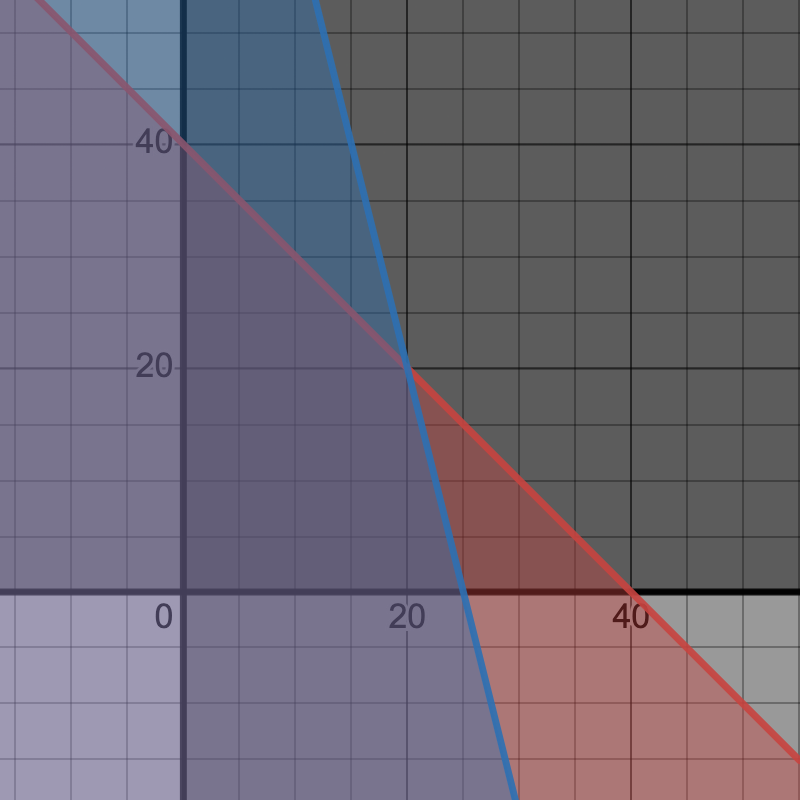
\includegraphics[width=0.4\textwidth]{01/01-chocolate_example_soln.png}
    \end{center}
    \caption{Graph from Desmos}\label{chocolate-graph}
\end{wrapfigure}
\textbf{Solution. } The simplest way to find the optimal solution to this problem
is through graphical methods. We can simply plot the constraints, locate the
overlapping/feasible region, plug in the coordinates of the angles
into $f$ and choose the best one. For this, we can use Desmos to plot the constraint
inequalities from Equation~\ref{chocolate-formulation}.

Notice that on Figure~\ref{chocolate-graph}, the feasible region is the irregular
rectangle where everything overlaps$-$essentially the $(20, 20)$ square plus some 
extrusions. From the plot, we can see that the angles are at $(0, 0), (0, 40), (25, 0)$,
and $(20, 20)$. We can plug each of these coordinates into the objective function 
to get $0, 40, 50$, and $60$ respectively. Therefore, we can conclude that producing 
20 units of each chocolate makes the most profit$-$a profit of \$60.

Additionally, since the coordinates we used are in the region where every constraint 
inequality overlap, we know that the solution that we have is valid.

Therefore, we can conclude that the optimal solution $(x^*, y^*)$ is $(20, 20)$ where
the optimal value $z^*$ is $60$.
\end{example}

\begin{example}
A bolts and nails factory is making bolts and nails where both needs to be turned,
grinded, and hand-adjusted by a human. The plant has 120, 36, and 80 hours of
turning, grinding, and manpower capacity per week respectively. \$13 profit is made
from every 1000 bolts and \$15 from every 1000 nails. The amount of resources needed 
to produce bolts and nails are described in the following table.

\begin{table}[H]
    \centering
    \begin{tabular}{|c|c|c|}
        \hline
        Activity & Number of hours per 1000 bolts & Number of hours per 1000 nails\\
        \hline
        Turning & 3 & 4\\
        Grinding & 2 & 1\\
        Manpower & 1 & 3\\
        \hline
    \end{tabular}
    \caption{Time resource required to produce bolts and nails}
\end{table}

The factory wants to find the number of bolts and nails they should produce weekly to 
maximize weekly profits. For this example, the model is the only thing identified.

\textbf{Formulation. } Let $x$ and $y$ be the number of bolts and nails produced weekly.
Note that the unit is 1000 units not just a unit by itself. Let the objective function 
represent the weekly profit.
\begin{equation}
    \begin{aligned}
        \max_{(x, y)} \quad & f(x, y) = 13x + 15y\\
        s.t. \quad & 3x + 4y \leq 120\\
        & 2x + y \leq 36\\
        & x + 3y \leq 80\\
        & x, y \geq 0
    \end{aligned}
\end{equation}
\end{example}

\subsection*{Slope of the Objective Function $f$}

In the previous example, we have two decision variables to consider. We also only have
two axes for plotting. So, we can do some manipulation to solve the problem a bit 
easier. First, recall the objective function: \[ f(x, y) = z = 2x + y \] From there, 
we can manipulate it to obtain 
\begin{equation}\label{slope-of-f}
y = -2x + z 
\end{equation}
where $z$ becomes an arbitrary parameter representing the y-intercept.

Notice how Equation~\ref{slope-of-f} becomes an equation of a line where the slope
is -2. From there, we can simply come up with an arbitrary value for $z$ and keep
changing it (increasing, for this problem) until the line is not in the feasible region 
anymore. With this method, our solution is simply the last point on the line that 
remains within the feasible region as we change $z$.

\section{Linear Programming Model}

Think of linear programming model as a subset of mathematical programming where it 
consists of optimization models where everything about it is linear. This means that
the objective function and the constraint equations or inequalities are linear, and 
that there could be a \textit{sign restriction} associated with each variable. In
most cases, they will either have a non-negative constraint have no sign restriction.

\subsection*{Linear Functions}

Linear functions refer to any function $f$ that has the form 
\[ f(x) = c_1x_1 + c_2x_2 + \cdots + c_n x_n \]
where each $x_i$ is a decision variable and each $c_i$ is a constant coefficient.

\subsection*{Linear Equations and Inequalities}

Given some arbitrary $b$ and a set of $a_i$, the equation or inequality must
come in the form of
\[ a_1x_1 + a_2x_2 + \cdots + a_n x_n \leq b \]
or
\[ a_1x_1 + a_2x_2 + \cdots + a_n x_n = b \]
where $b$ is some arbitrary value and $a_i$ is a constant coefficient for each
decision variable $x_i$.

\section{Linear Programming Assumptions}

In linear programming, there are a few assumptions we make in order to make solving
the problem simpler. These assumptions are the following

\subsection*{Proportionality}

Contribution of each decision variable to the objective function and constraints is 
proportional. For example, suppose that you need $n$ hours to create $x$ units of
an item, you will need $3n$ hours to create $3x$ units of the same item.

Note that this assumption falls apart when the economy of scale is introduced since 
there are proportional savings gained from increased production. This will be covered 
later on.

\subsection*{Additivity}

Individual contributions of different decision variables can be \textit{summed} up to 
obtain an objective function and constraint. This implies that whatever computation
you do on the decision variable in the objective function, you will end up with the
same unit. For example, the total time for producing two kinds of products is the sum 
of the amount of time it takes to produce each product.

\subsection*{Certainty}

Each parameter$-$essentially any data or value that is given to us$-$ is known for sure.
There is no randomness in these parameters.

\subsection*{Divisibility}

Decision variables must be able to take the form of an integer \textit{as well as
fractional values}. For example, decision variable $x$ could be both $3.1415$ or $2$,
depending on the case.